\documentclass[11pt]{article}

\usepackage[a4paper,margin=1in]{geometry}
\usepackage{graphicx}
\usepackage{booktabs}
\usepackage{amsmath}
\usepackage{siunitx}
\usepackage{caption}
\usepackage{subcaption}
\usepackage{float}
\usepackage[hidelinks]{hyperref}

\graphicspath{{../figures/}{figures/}}

\title{Adversarial Search in Isolation:\\Minimax vs.\ Alpha-Beta Pruning}
\author{Amr Yasser}
\date{\today}

\begin{document}
\maketitle

\begin{abstract}
This project implements the game \textit{Isolation} and compares two adversarial search algorithms:
Minimax and Alpha-Beta pruning. We evaluate them under controlled conditions (same depth),
under realistic constraints (same time budget via iterative deepening), and in gameplay against a
random baseline. We also demonstrate a critical practical insight: Alpha-Beta pruning effectiveness
depends strongly on move ordering. Results show that Alpha-Beta expands far fewer nodes than
Minimax at the same depth, and with good move ordering can reduce expansions dramatically.
\end{abstract}

\section{Introduction}
Adversarial search is a core technique for decision-making in deterministic, turn-based, perfect-information games.
Minimax provides an optimal decision rule (under a depth limit and heuristic evaluation).
Alpha-Beta pruning is an optimization that returns the same move as Minimax at a fixed depth, but can avoid
exploring large parts of the game tree.

This report covers:
\begin{itemize}
  \item the Isolation game, including state representation, actions, and transition function,
  \item Minimax and Alpha-Beta in simple terms,
  \item the evaluation function used,
  \item experimental results: time, nodes explored, and depth reached,
  \item reflections on observed behavior and efficiency.
\end{itemize}

\section{Game: Isolation}
\subsection{State representation}
A state \(s\) stores:
\begin{itemize}
  \item a board grid where each cell is empty, blocked, or occupied by \(A\) or \(B\),
  \item the current position of each player (or \texttt{None} before initial placement),
  \item the active player (whose turn it is).
\end{itemize}

\subsection{Initial state}
The initial state is an empty board (no blocks) with both player positions unset. The first time each player moves,
they \textbf{place} their piece on any empty cell.

\subsection{Actions (legal moves)}
Let the active player be \(p\) with current position \((r,c)\).
\begin{itemize}
  \item If \(p\) has not been placed yet, the action set is all empty cells.
  \item Otherwise, an action is a \textbf{queen move}: slide any number of squares in one of 8 directions
  (horizontal/vertical/diagonal) until blocked/occupied.
\end{itemize}

\subsection{Transition function}
Given a state \(s\) and action \(a\) (a destination cell), the transition \(T(s,a)=s'\) is:
\begin{itemize}
  \item move the active player to \(a\),
  \item mark the previous player cell as blocked (unusable),
  \item switch the active player.
\end{itemize}

\subsection{Terminal states}
A state is terminal if the active player has \textbf{no legal actions}. The player to move loses; equivalently,
the winner is the opponent of the active player in the terminal state.

\section{Algorithms}
\subsection{Minimax (depth-limited)}
Minimax searches a game tree to depth \(d\), alternating:
\begin{itemize}
  \item \textbf{max} levels: choose the move that maximizes utility for the root player,
  \item \textbf{min} levels: choose the move that minimizes utility (opponent response).
\end{itemize}
At depth \(0\) or terminal states, a heuristic evaluation estimates utility.

\subsection{Alpha-Beta pruning}
Alpha-Beta pruning returns the same move/value as Minimax at a fixed depth, but maintains:
\begin{itemize}
  \item \(\alpha\): best value found so far for the maximizing player,
  \item \(\beta\): best value found so far for the minimizing player.
\end{itemize}
If \(\alpha \ge \beta\), the remaining sibling branches cannot affect the final choice and are pruned.

\subsection{Evaluation function}
We use a standard Isolation heuristic: \textbf{mobility difference}
\[
h(s) = \#\text{legal moves for root} - \#\text{legal moves for opponent}.
\]
This is suitable for Isolation because the game is fundamentally about restricting the opponent's mobility.
Terminal states return large-magnitude utilities so that forced wins/losses dominate heuristic estimates.

\subsection{Iterative deepening and ``depth reached''}
Under a per-move time budget, the agents use iterative deepening: search depth \(1,2,\dots\) until time runs out.
We record \textbf{depth reached} as the deepest fully-completed depth within the budget for that move.

\section{Experimental Methodology}
\begin{itemize}
  \item \textbf{Setup A (same depth):} compare Minimax vs Alpha-Beta fairly at identical depth on identical states.
  \item \textbf{Setup B (same time):} compare behavior under a fixed time budget and record depth reached.
  \item \textbf{Setup C (vs random):} measure win rate and efficiency in gameplay against a random baseline.
  \item \textbf{Setup D (move ordering):} isolate the impact of move ordering on Alpha-Beta pruning.
\end{itemize}

\section{Results}
\subsection{Setup A (same depth): nodes and time}
\begin{figure}[H]
  \centering
  \begin{subcaptionbox}{Average nodes expanded (same depth)\label{fig:setupA_nodes}}
    {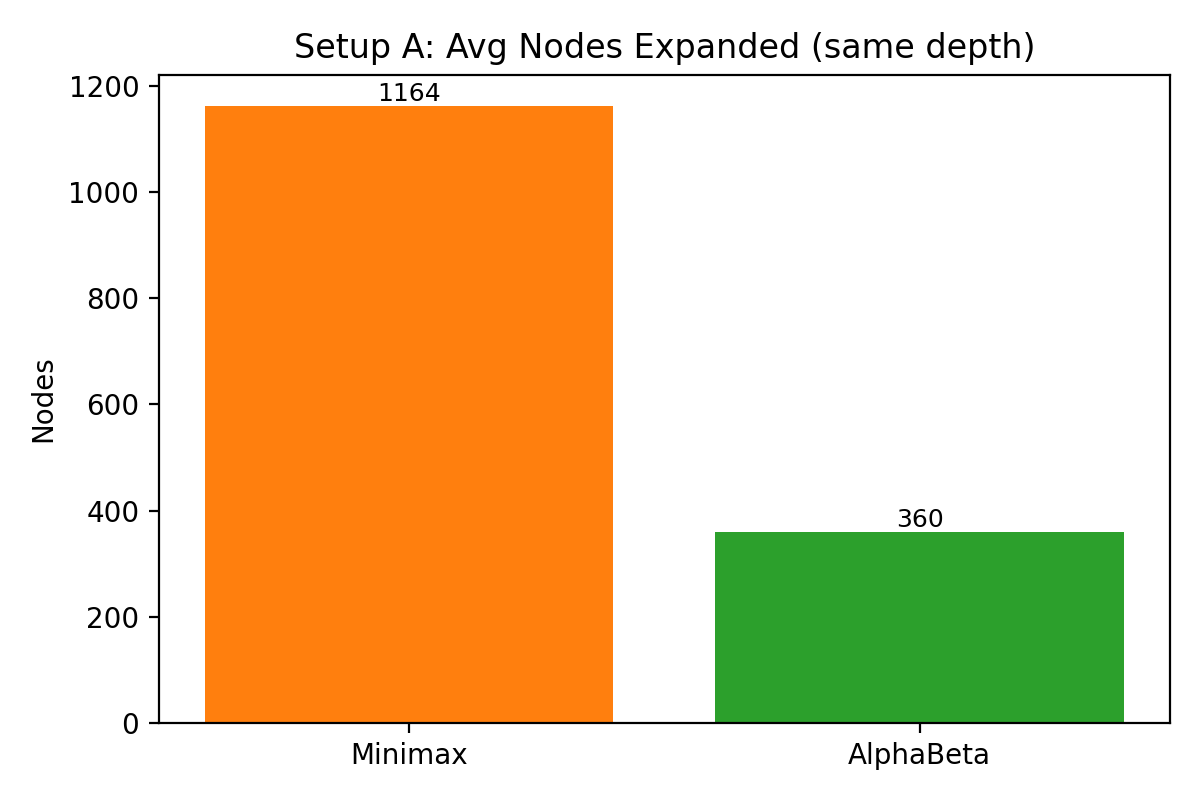
\includegraphics[width=0.48\textwidth]{setupA_nodes.png}}
  \end{subcaptionbox}\hfill
  \begin{subcaptionbox}{Average runtime (same depth)\label{fig:setupA_time}}
    {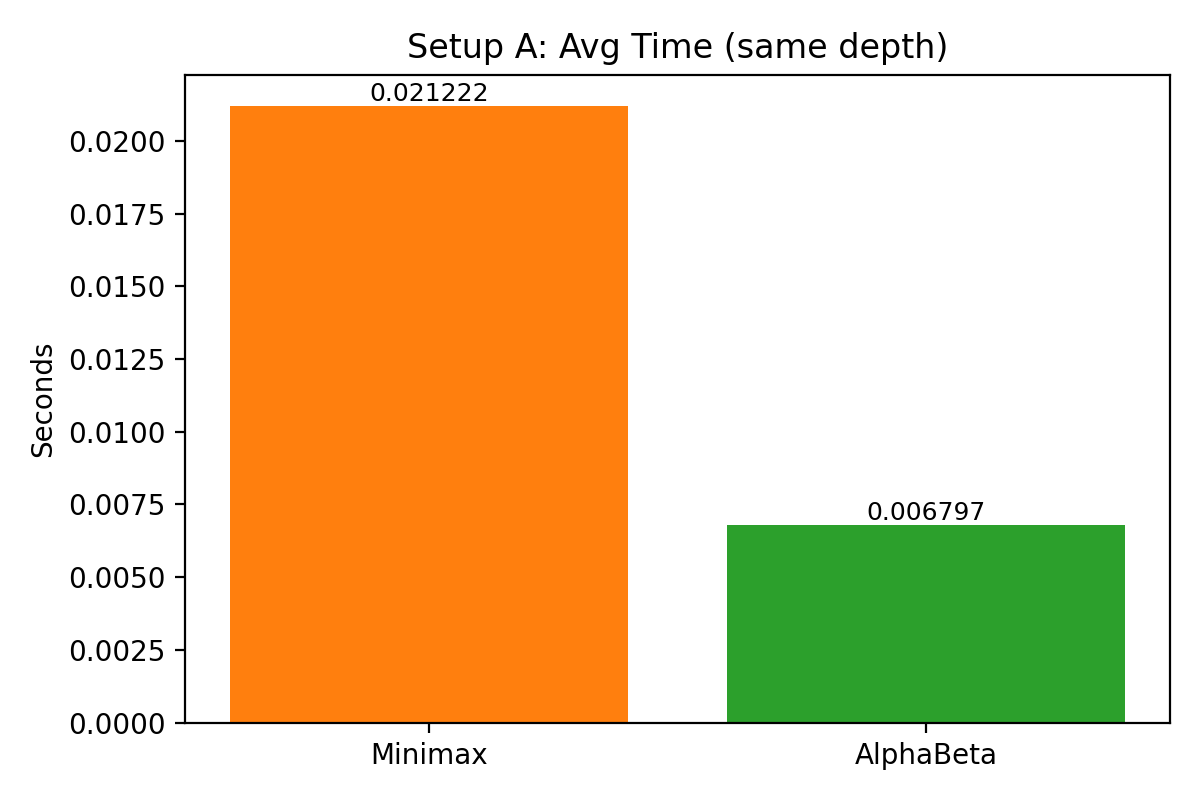
\includegraphics[width=0.48\textwidth]{setupA_time.png}}
  \end{subcaptionbox}
  \caption{Setup A: Alpha-Beta expands fewer nodes and runs faster than Minimax at the same depth.}
\end{figure}

\subsection{Setup B (same time): depth reached}
\begin{figure}[H]
  \centering
  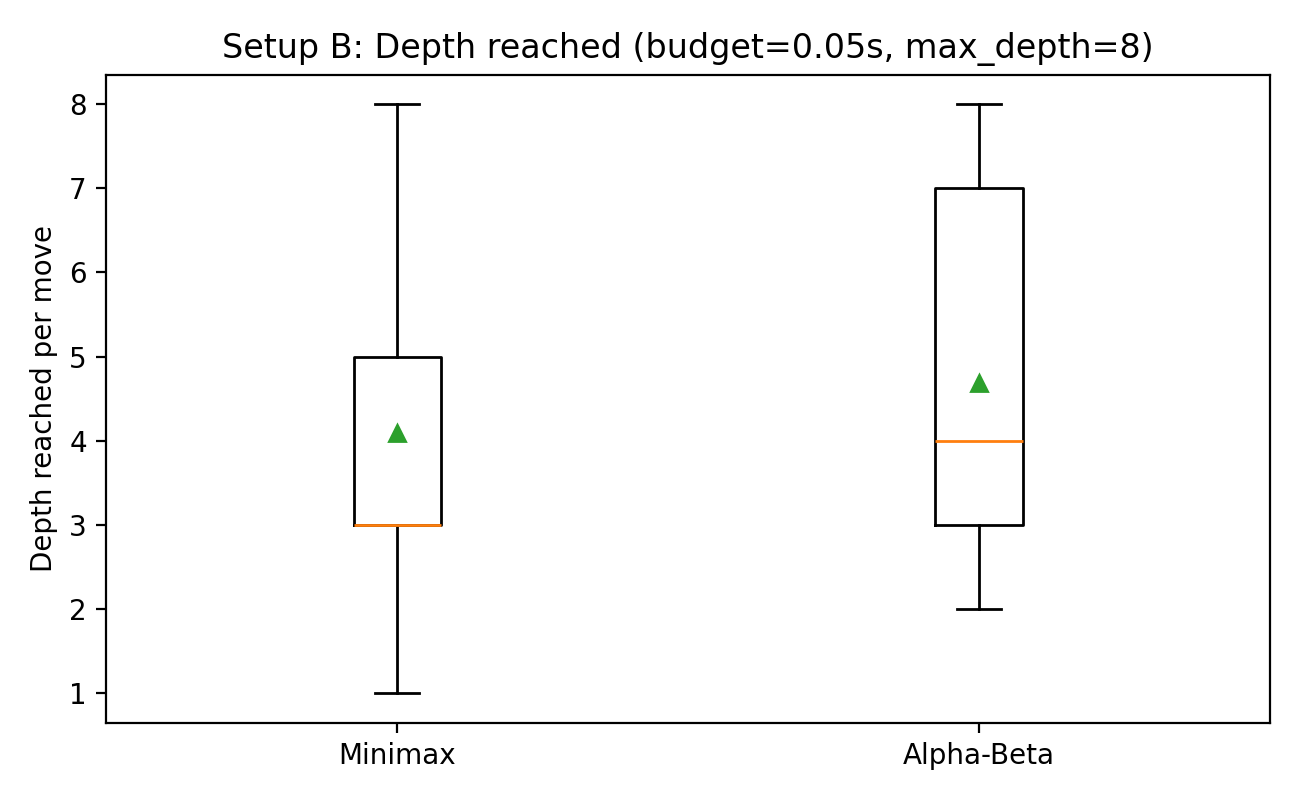
\includegraphics[width=0.70\textwidth]{setupB_depth.png}
  \caption{Setup B: Depth reached per move under the same time budget using iterative deepening (mean shown).}
  \label{fig:setupB_depth}
\end{figure}

\noindent This directly quantifies how pruning translates into deeper search under a time constraint.

\subsection{Setup C (fixed depth vs random): wins, nodes/move, time/move}
\begin{figure}[H]
  \centering
  \begin{subcaptionbox}{Win rate vs random\label{fig:setupC_wins}}
    {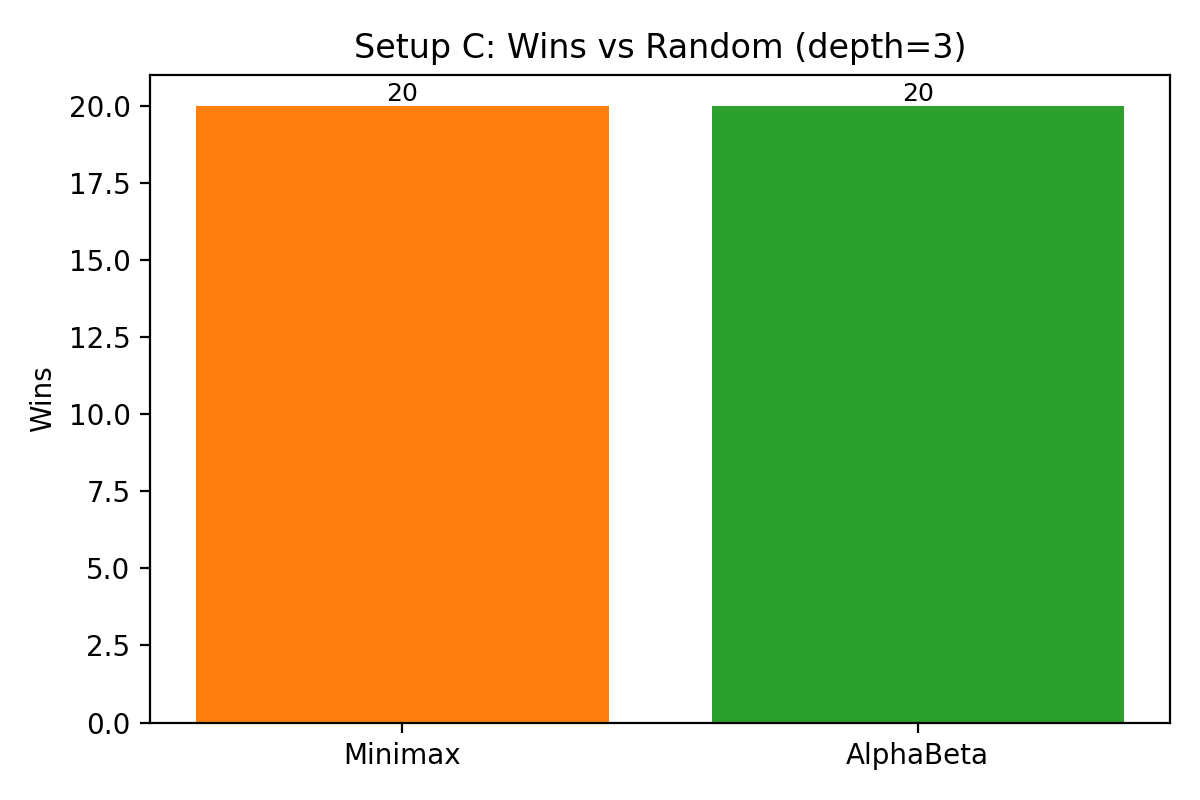
\includegraphics[width=0.32\textwidth]{setupC_wins.png}}
  \end{subcaptionbox}\hfill
  \begin{subcaptionbox}{Avg.\ nodes per move\label{fig:setupC_nodes}}
    {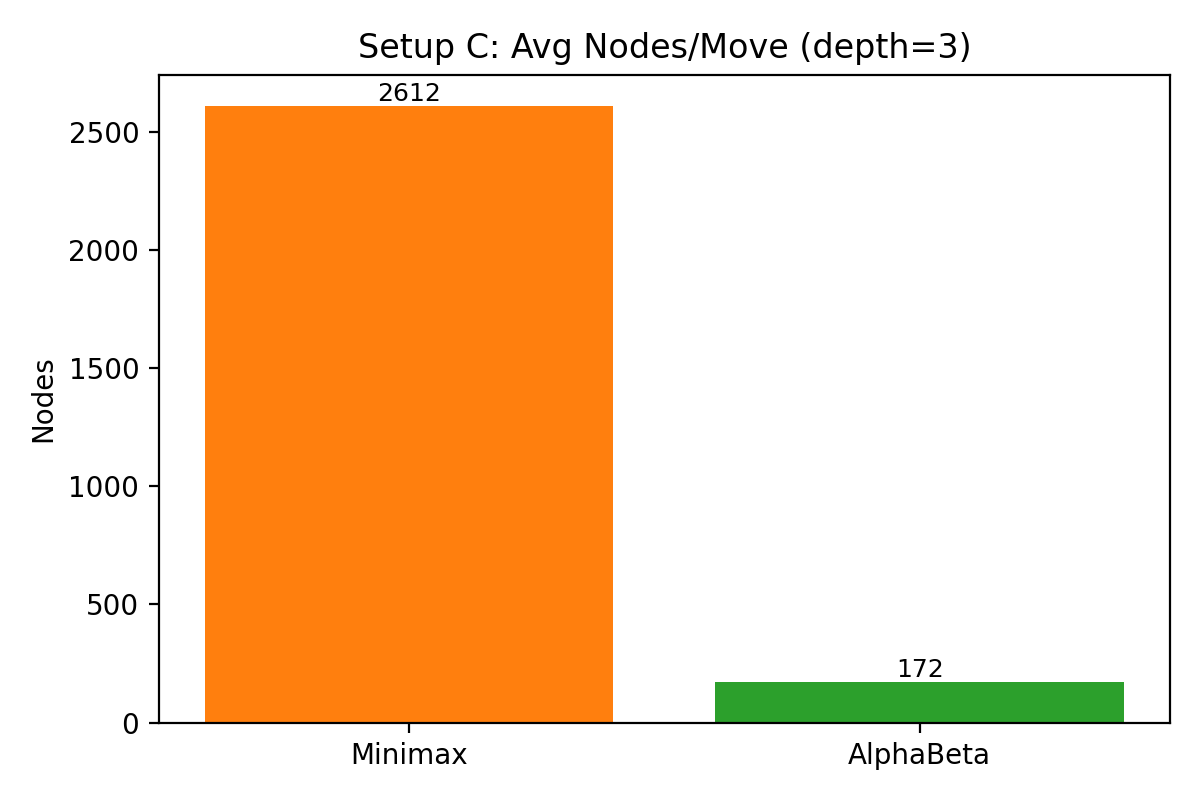
\includegraphics[width=0.32\textwidth]{setupC_nodes.png}}
  \end{subcaptionbox}\hfill
  \begin{subcaptionbox}{Avg.\ time per move\label{fig:setupC_time}}
    {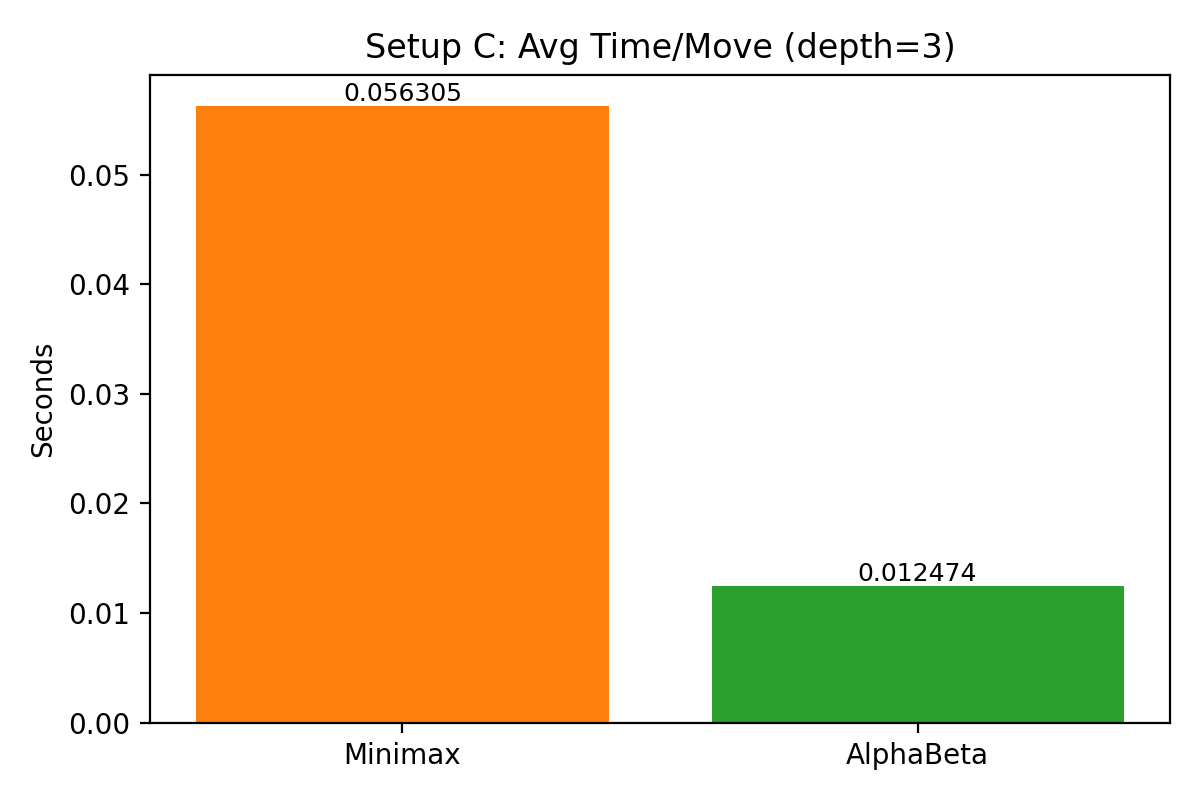
\includegraphics[width=0.32\textwidth]{setupC_time.png}}
  \end{subcaptionbox}
  \caption{Setup C: Against random play, both search agents win reliably, while Alpha-Beta is significantly more efficient.}
\end{figure}

\subsection{Setup D (move ordering impact): nodes, cutoffs, and pruned tree}
\begin{figure}[H]
  \centering
  \begin{subcaptionbox}{Nodes expanded\label{fig:setupD_nodes}}
    {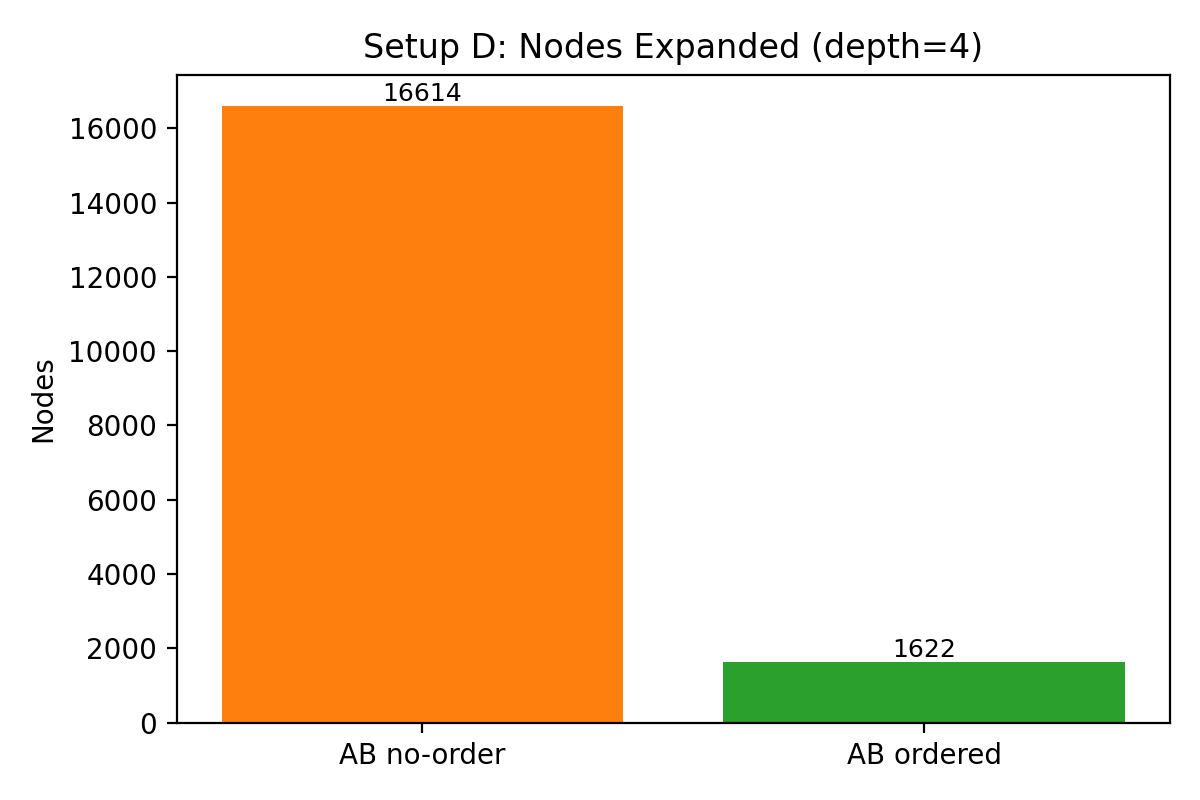
\includegraphics[width=0.48\textwidth]{setupD_nodes.png}}
  \end{subcaptionbox}\hfill
  \begin{subcaptionbox}{Cutoffs\label{fig:setupD_cutoffs}}
    {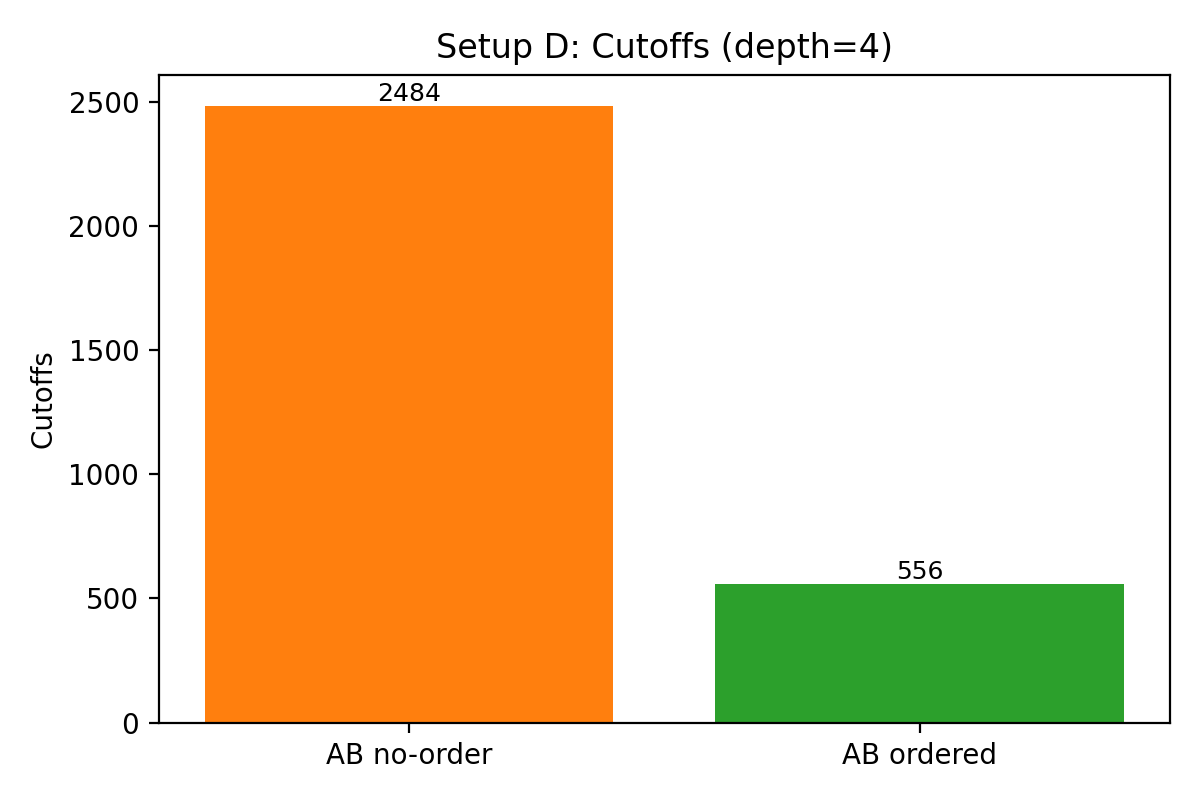
\includegraphics[width=0.48\textwidth]{setupD_cutoffs.png}}
  \end{subcaptionbox}
  \caption{Setup D: Move ordering significantly increases Alpha-Beta pruning effectiveness.}
\end{figure}

\begin{figure}[H]
  \centering
  \begin{subcaptionbox}{Example start state\label{fig:setupD_board}}
    {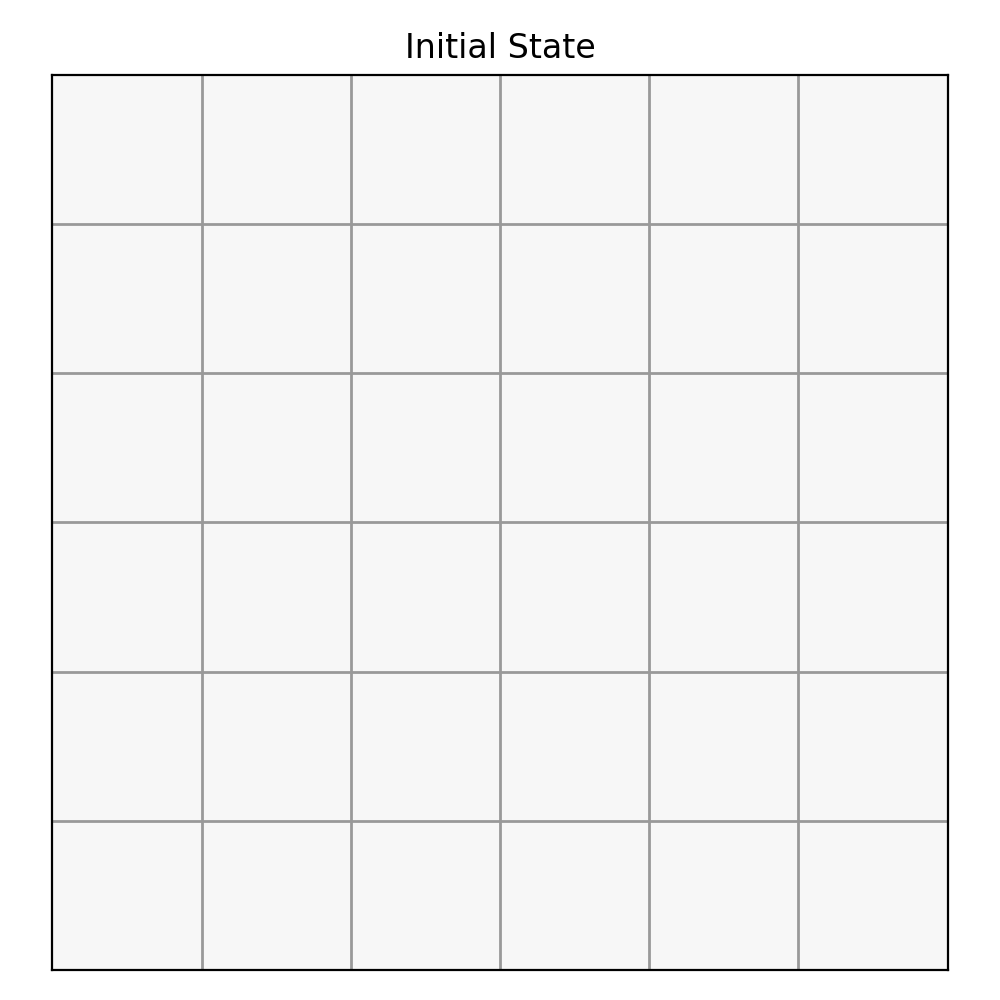
\includegraphics[width=0.32\textwidth]{setupD_initial_board.png}}
  \end{subcaptionbox}\hfill
  \begin{subcaptionbox}{Partial search tree with pruned branches\label{fig:setupD_tree}}
    {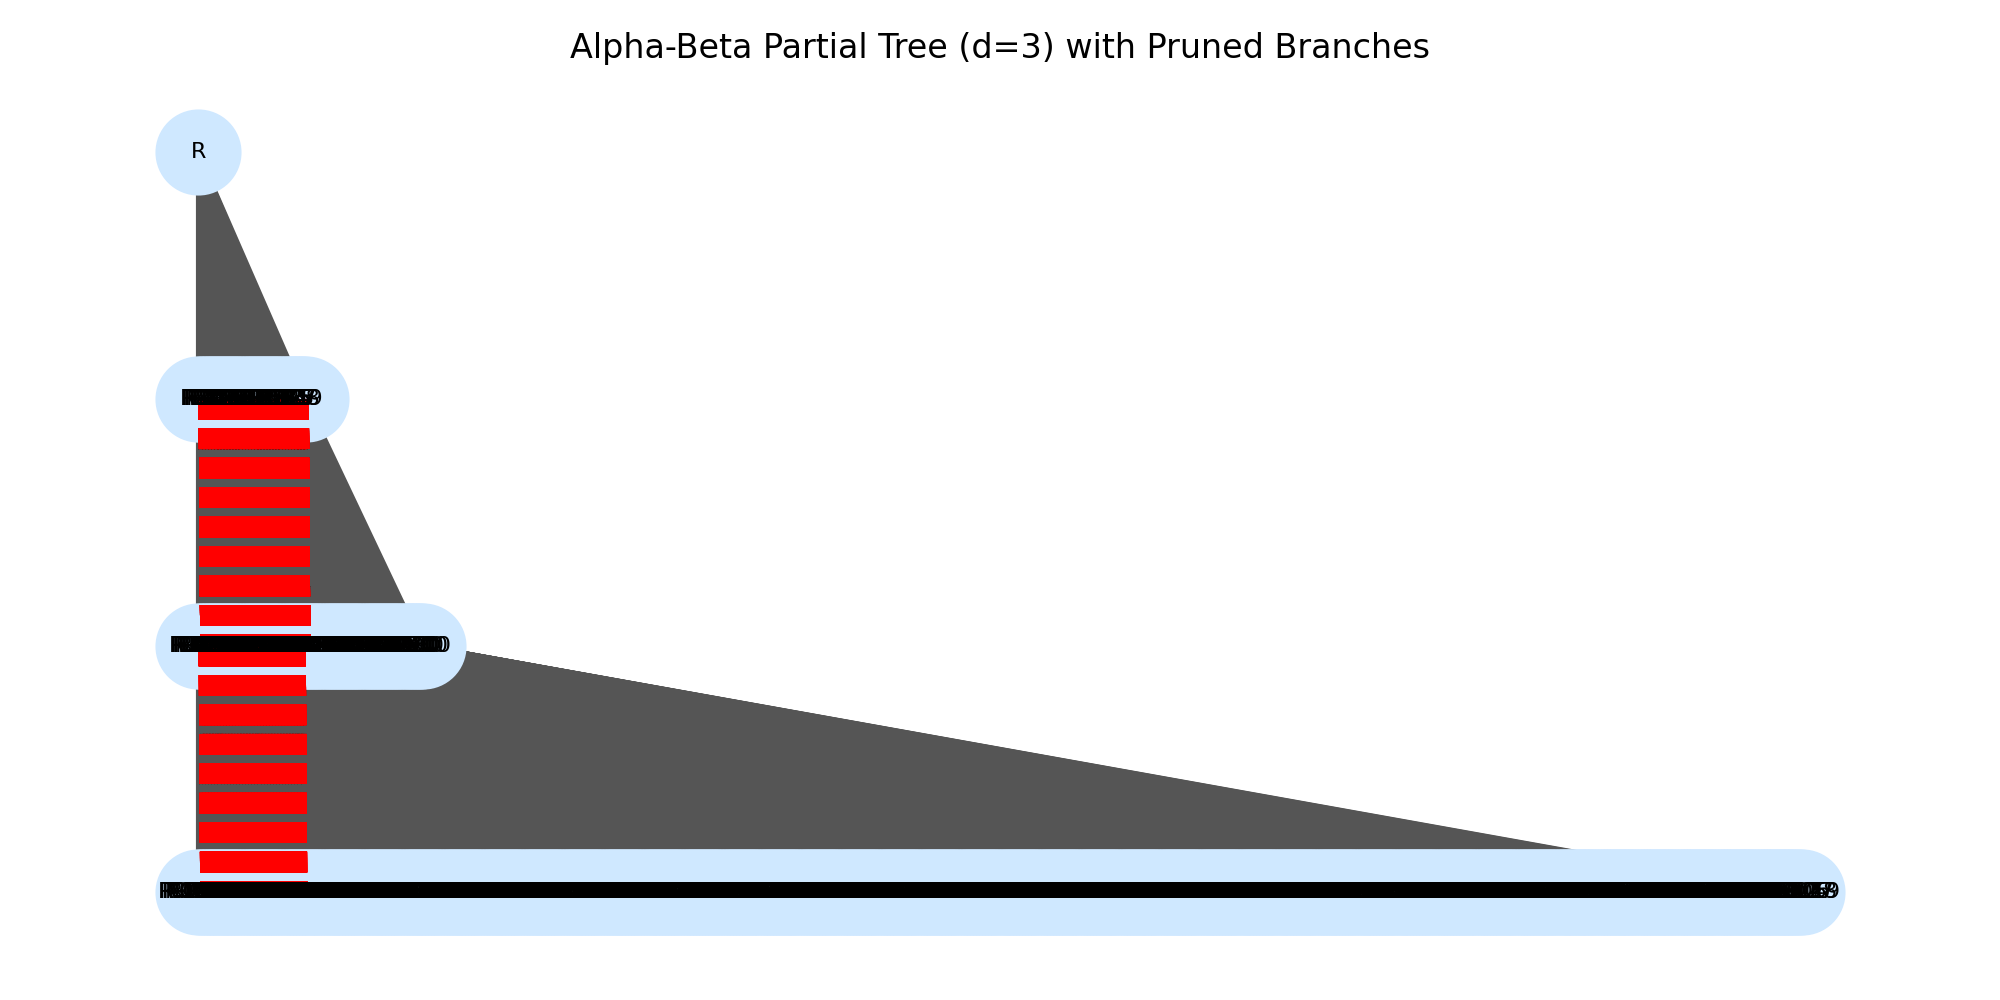
\includegraphics[width=0.64\textwidth]{setupD_pruned_tree.png}}
  \end{subcaptionbox}
  \caption{Visualization of Alpha-Beta pruning (ordered). Pruned branches are omitted/marked.}
\end{figure}

\section{Qualitative Gameplay Snapshots}
\begin{figure}[H]
  \centering
  \begin{subcaptionbox}{Initial placement phase}
    {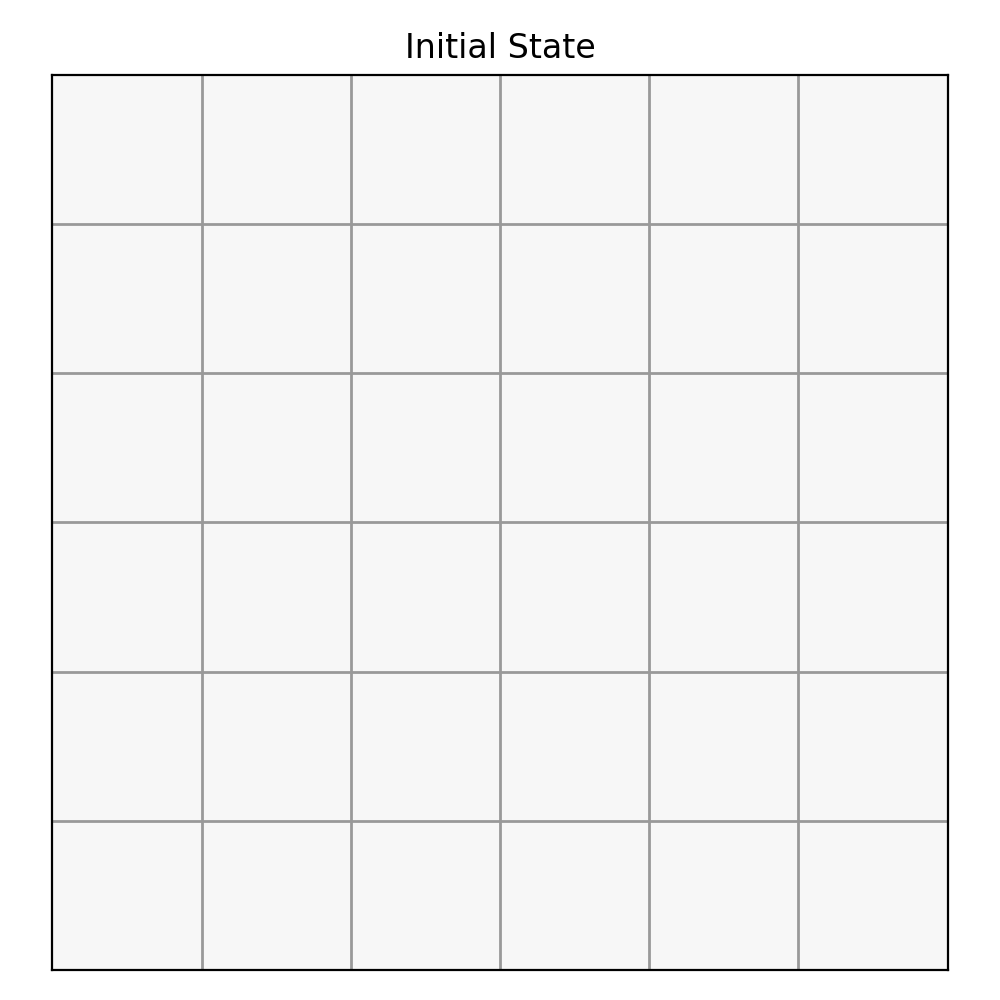
\includegraphics[width=0.48\textwidth]{ab_vs_random_00.png}}
  \end{subcaptionbox}\hfill
  \begin{subcaptionbox}{Later state after several plies}
    {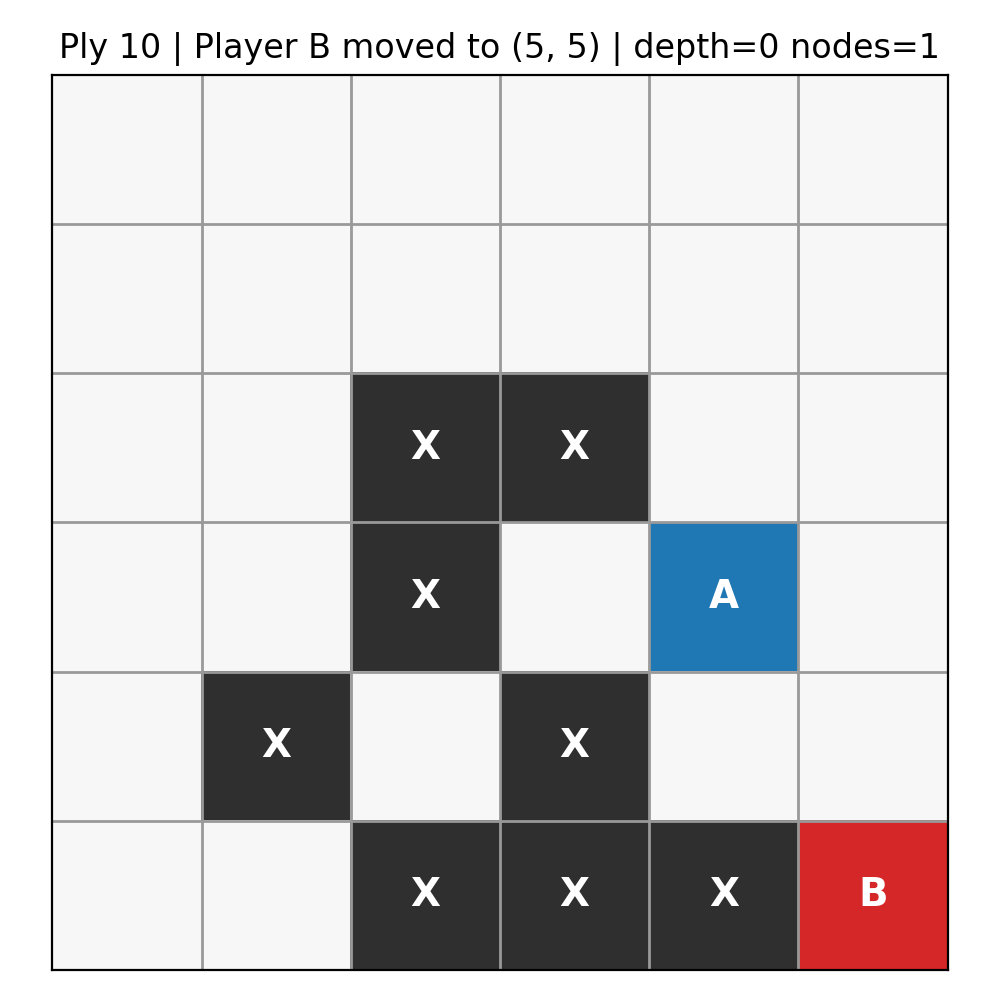
\includegraphics[width=0.48\textwidth]{ab_vs_random_10.png}}
  \end{subcaptionbox}
  \caption{Two snapshots from Alpha-Beta vs Random. Blocked squares accumulate as pieces move.}
\end{figure}

\section{Reflections and Observations}
\begin{itemize}
  \item \textbf{Efficiency vs strength:} At fixed depth, Alpha-Beta mainly improves efficiency (fewer nodes/time).
  Under time limits, the same efficiency often converts to \textbf{greater depth reached} (Fig.~\ref{fig:setupB_depth}),
  which can improve playing strength against non-trivial opponents.
  \item \textbf{Move ordering matters:} Alpha-Beta pruning can range from modest to dramatic depending on move ordering,
  as shown by node and cutoff differences in Setup D.
  \item \textbf{Heuristic suitability:} Mobility difference is a natural fit for Isolation because the win condition is
  directly tied to restricting legal moves. It is simple, fast, and effective for depth-limited search.
\end{itemize}

\section{Reproducibility}
From the project root:
\begin{itemize}
  \item Run tests: \texttt{python -m pytest -q}
  \item Run experiments (A--D): \texttt{python -m experiments.run\_setups}
  \item Generate all figures + snapshots: \texttt{python -m visualization.auto\_generate\_figures}
\end{itemize}

\end{document}